\documentclass[11pt]{article}
\usepackage[margin=1in]{geometry}
\usepackage{amsmath,amssymb}
\usepackage{booktabs}
\usepackage{xcolor}
\usepackage{hyperref}

\usepackage{tikz}
\usetikzlibrary{shapes.geometric,arrows.meta,positioning,fit,backgrounds}
\usepackage{longtable}
\usepackage{caption}
\usepackage{tabularx}
\usepackage{graphicx}
\hypersetup{colorlinks=true,linkcolor=blue!50!black,citecolor=blue!50!black,urlcolor=blue!50!black}
\sloppy

\newcommand{\good}{\textcolor{green!50!black}{\textbf{Feasible}}}
\newcommand{\risky}{\textcolor{orange!80!black}{\textbf{Feasible, higher risk}}}
\newcommand{\hard}{\textcolor{red!70!black}{\textbf{Resource-limited}}}

\title{\textbf{Cross-Modal Emotion-Aligned Latent Space for\\ Video/Text-Conditioned Music Generation}\\
\large Feasibility Assessment and Implementation Plan}
\author{EmoMV Project}
\date{\today}

\begin{document}
\maketitle
\tableofcontents

\section*{Executive Summary}
\addcontentsline{toc}{section}{Executive Summary}

You currently have two independently trained, frozen-backbone \textbf{5-class mood classifiers} —
a video model (VideoMAE + CLIP $\to$ fusion head, 80.1\% test accuracy) and a text model
(fine-tuned DistilRoBERTa, macro-F1 $\approx 0.80$). The proposed next phase is to bolt a small
\emph{projection adapter} onto each frozen encoder and train the two adapters jointly with a
contrastive (InfoNCE/CLIP-style) loss, producing a shared, modality-agnostic embedding space.
That space would later condition a fine-tuned MusicGen model to generate music from video or text
input.

\textbf{Verdict: the overall project is feasible in phases, and the next phase (cross-modal
alignment) is straightforward with the resources you already have.} The one design decision that
materially changes the approach — and the central finding of this document — is that
\textbf{you do not have literal (video, caption) pairs to train a standard CLIP-style
contrastive loss on}. What you have instead is two datasets that each carry the \emph{same
5-class categorical label}. Section~\ref{sec:pairing} explains why this is still workable (a
well-established technique, \emph{label-anchored supervised contrastive alignment}), what it
gives you, and what it does \emph{not} give you. Section~\ref{sec:musicgen} identifies a
resource you already have and may not have noticed: because your video encoder was trained only
on EmoMV's \texttt{MATCH} clips (video emotion~=~music emotion, by the dataset's own
construction), \textbf{every one of your 3{,}178 training clips already has a mood-consistent
music track attached} — which is exactly the paired data Stage~C needs.

\begin{center}
\begin{tabularx}{\textwidth}{@{}X l X@{}}
\toprule
\textbf{Stage} & \textbf{Status} & \textbf{Feasibility on your current hardware} \\
\midrule
A. Unimodal classifiers (video, text) & Done & --- \\
B. Cross-modal projection + contrastive alignment & Proposed next & \good \\
C. MusicGen conditioning / fine-tuning & Future & \risky\ (compute risk on Apple Silicon) \\
\bottomrule
\end{tabularx}
\end{center}

\section{Current Assets}

\subsection{Video encoder (Stage A, done)}
Built and evaluated in the EmoMV preprocessing/training pipeline (\texttt{project/}): frozen
\texttt{VideoMAE-base} (768-d, mean-pooled) $+$ frozen \texttt{CLIP ViT-B/32} (512-d, mean-pooled
over 16 frames) $\to$ concatenated 1280-d vector $\to$ trained fusion head
(\texttt{Linear(1280,512)} $\to$ GELU $\to$ Dropout $\to$ \texttt{Linear(512,5)}).

\begin{center}
\begin{tabular}{@{}lrrr@{}}
\toprule
& Accuracy & Macro-F1 & Weighted-F1 \\
\midrule
SlowFast baseline (reference) & 50.6\% & 0.479 & 0.503 \\
\textbf{VideoMAE+CLIP fusion (current video model)} & \textbf{80.1\%} & \textbf{0.794} & \textbf{0.803} \\
\bottomrule
\end{tabular}
\end{center}

\textbf{Important terminology note.} The VideoMAE and CLIP \emph{backbones themselves are frozen}
— only the 512-d fusion head was trained. What you have is not a fine-tuned encoder in the
strict sense (no gradients ever reached VideoMAE/CLIP's weights); it is a frozen general-purpose
representation plus a small trained classification head. This distinction does not block Stage~B
— in fact it is the \emph{recommended} pattern for exactly this kind of adapter-based alignment
(Section~\ref{sec:embedding-choice}) — but it is worth being precise about when writing this up,
since "fine-tuned video encoder" and "frozen encoder with a trained head" have different
implications for how much the representation has actually specialized to your 5 mood classes.

\subsection{Text encoder (Stage A, done)}
Located at \texttt{project/text\_mood\_clf\_encoder/}: \texttt{distilroberta-base}
(\texttt{RobertaForSequenceClassification}, 6 transformer layers, hidden size 768, 12 attention
heads, vocab 50{,}265) \textbf{fully fine-tuned} end-to-end for 5-class mood classification. Test
macro-F1 $\approx 0.80$. Unlike the video model, this is a genuine fine-tuned encoder — the
RoBERTa backbone's own weights were updated during training.

\begin{center}
\begin{tabular}{@{}lrl@{}}
\toprule
\textbf{id} & \textbf{video label} & \textbf{text label} \\
\midrule
0 & exciting & excited \\
1 & fear & fear \\
2 & tense & tense \\
3 & sad & sad \\
4 & relax & relax \\
\bottomrule
\end{tabular}
\end{center}

The label ordering is identical between the two encoders (only "exciting" vs. "excited" differs
lexically) — a small but genuinely useful coincidence: any code that treats labels as integer
class IDs 0--4 does not need a remapping table between the two encoders.

\section{Proposed System Overview}

\begin{center}
\resizebox{\textwidth}{!}{%
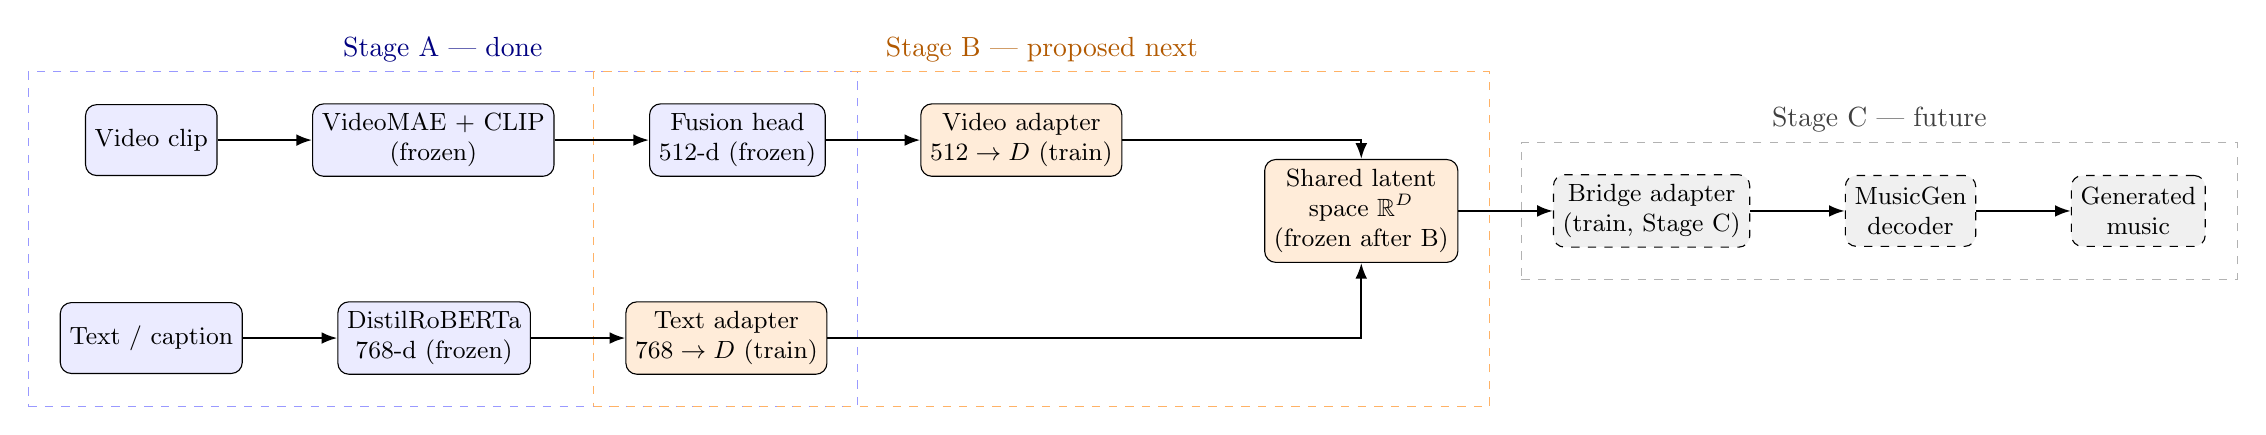
\begin{tikzpicture}[
  node distance=8mm and 12mm,
  box/.style={rectangle, draw, rounded corners, minimum height=9mm, align=center, font=\small},
  frozen/.style={box, fill=blue!8},
  train/.style={box, fill=orange!15},
  future/.style={box, fill=gray!12, dashed},
  arr/.style={-{Latex[length=2mm]}, thick}
]

% Stage A/B - video branch
\node[frozen] (vid) {Video clip};
\node[frozen, right=of vid] (vmae) {VideoMAE + CLIP\\(frozen)};
\node[frozen, right=of vmae] (vhead) {Fusion head\\512-d (frozen)};
\node[train, right=of vhead] (vadapt) {Video adapter\\$512 \to D$ (train)};

% Stage A/B - text branch
\node[frozen, below=16mm of vid] (txt) {Text / caption};
\node[frozen, right=of txt] (roberta) {DistilRoBERTa\\768-d (frozen)};
\node[train, right=of roberta] (tadapt) {Text adapter\\$768 \to D$ (train)};

% Shared space
\node[train, right=18mm of vadapt, yshift=-9mm] (shared) {Shared latent\\space $\mathbb{R}^D$\\(frozen after B)};

% Stage C
\node[future, right=of shared] (bridge) {Bridge adapter\\(train, Stage C)};
\node[future, right=of bridge] (musicgen) {MusicGen\\decoder};
\node[future, right=of musicgen] (music) {Generated\\music};

\draw[arr] (vid) -- (vmae);
\draw[arr] (vmae) -- (vhead);
\draw[arr] (vhead) -- (vadapt);
\draw[arr] (txt) -- (roberta);
\draw[arr] (roberta) -- (tadapt);
\draw[arr] (vadapt.east) -| (shared.north);
\draw[arr] (tadapt.east) -| (shared.south);
\draw[arr] (shared) -- (bridge);
\draw[arr] (bridge) -- (musicgen);
\draw[arr] (musicgen) -- (music);

\begin{scope}[on background layer]
\node[fit=(vid)(vmae)(vhead)(txt)(roberta), draw=blue!40, dashed, inner sep=4mm, label={[blue!50!black]above:Stage A --- done}] {};
\node[fit=(vadapt)(tadapt)(shared), draw=orange!60, dashed, inner sep=4mm, label={[orange!70!black]above:Stage B --- proposed next}] {};
\node[fit=(bridge)(musicgen)(music), draw=gray!60, dashed, inner sep=4mm, label={[gray!50!black]above:Stage C --- future}] {};
\end{scope}
\end{tikzpicture}%
}
\end{center}

Blue = already frozen/trained. Orange = the next thing to train (small, cheap). Gray/dashed =
future work, contingent on Stage B succeeding.

\section{Stage B: Cross-Modal Alignment}

\subsection{Which embedding to project}
\label{sec:embedding-choice}
Do not project the raw 1280-d concatenated VideoMAE+CLIP vector, and do not project RoBERTa's raw
token embeddings. Project the \emph{penultimate, task-supervised} representation from each
existing classifier:

\begin{itemize}
\item \textbf{Video:} the 512-d activation after \texttt{Linear(1280,512)} $\to$ GELU $\to$
Dropout, i.e. everything in \texttt{FusionClassifier} except the final \texttt{Linear(512,5)}.
\item \textbf{Text:} the 768-d pooled/CLS representation RoBERTa's classification head consumes,
i.e. everything in \texttt{RobertaClassificationHead} except the final \texttt{out\_proj}.
\end{itemize}

Both are already the result of \emph{supervised} training toward the same 5-class taxonomy, so
they start Stage~B already partially aligned in a semantic (if not geometric) sense — the
projection adapters have to learn a much easier function (a geometric alignment of two
already-discriminative spaces) than if they started from generic, task-agnostic backbone
features.

\subsection{Adapter architecture}
Two small MLPs, symmetric in design, asymmetric in input width:
\[
\text{video\_adapter}: \mathbb{R}^{512} \to \mathbb{R}^{D}, \qquad
\text{text\_adapter}: \mathbb{R}^{768} \to \mathbb{R}^{D}
\]
each implemented as \texttt{Linear(in,~2D)} $\to$ \texttt{LayerNorm} $\to$ GELU $\to$
\texttt{Dropout(0.1--0.2)} $\to$ \texttt{Linear(2D,~D)}, followed by L2 normalization
($\hat{z} = z / \lVert z \rVert_2$) so all downstream similarities are pure cosine similarities —
the same design CLIP itself uses.

\paragraph{Choosing $D$.} With only 3{,}178 video clips and a text-side dataset of unknown but
likely comparable order of magnitude, a smaller shared space regularizes better.

\begin{center}
\begin{tabularx}{\textwidth}{@{}X X X@{}}
\toprule
& $D=256$ (recommended start) & $D=512$ \\
\midrule
Overfitting risk & Lower & Higher on this data volume \\
Capacity for nuance beyond 5 classes & Lower & Higher \\
MusicGen bridge (Stage C) input & Smaller, simpler & Larger, more capacity \\
\bottomrule
\end{tabularx}
\end{center}
Start at $D=256$; only move to 512 if retrieval metrics (Section~\ref{sec:eval}) plateau below
what a linear probe on the raw 512-/768-d features already achieves — that would indicate the
adapters are under-capacity, not that the data is exhausted.

\subsection{The core feasibility question: what counts as a ``pair''?}
\label{sec:pairing}
Standard CLIP training relies on naturally occurring (image, caption) pairs — millions of them —
where each caption \emph{describes that specific image}. \textbf{You do not have this.} You have:

\begin{itemize}
\item $\sim$3{,}178 videos, each with one of 5 categorical mood labels.
\item An unknown-but-likely-larger text corpus, each sentence with one of the same 5 categorical
mood labels.
\item No instance-level correspondence between any specific video and any specific sentence.
\end{itemize}

This rules out literal CLIP-style pairing, but it does \emph{not} rule out contrastive alignment.
The applicable technique is \textbf{label-anchored supervised contrastive learning}
(a cross-modal generalization of Khosla et al., \emph{Supervised Contrastive Learning}, 2020):
within a training batch, treat \emph{any} text sample sharing a video sample's label as a
positive, and everything else as a negative. This is a well-established, correct way to train a
contrastive objective when you have shared categorical supervision instead of instance-level
pairs — it is, in effect, what you would get if you naively used class names as captions
(a technique CLIP itself uses at \emph{inference} time for zero-shot classification), generalized
to use your own, richer, label-consistent example sentences instead of a single class-name
string per class.

\textbf{What this buys you:} a shared space where "a video labeled \emph{relax}" and "a sentence
labeled \emph{relax}" land near each other, and the five mood clusters are well separated across
both modalities.

\textbf{What this does \emph{not} buy you:} fine-grained semantic alignment within a class. Two
very different relaxing scenes (a rainy evening with tea vs.\ a quiet mountain hike) will be
pulled to nearly the same point in the shared space, because the only training signal they share
is the class label \emph{relax}. If your downstream goal is coarse mood-conditioned generation
("make it feel relaxing"), this is entirely sufficient. If you eventually want the shared space to
distinguish \emph{shades} of relaxation, you will need richer supervision than 5 discrete labels
(e.g.\ LLM-generated per-clip captions used as weak paired text, or human-written descriptions) —
worth flagging now as a scoped-out stretch goal, not a blocker for Stage~B.

\subsection{Loss function}
For a batch of $N$ video embeddings $\{v_i\}$ and $N$ text embeddings $\{t_j\}$ (both
L2-normalized), with a learnable temperature $\tau$ (parameterized as CLIP does, via
$\text{logit\_scale} = \log(1/\tau)$, clamped to $[\log 1, \log 100]$):
\[
s_{ij} = \frac{v_i \cdot t_j}{\tau}
\]

\textbf{Simple (single-positive) InfoNCE}, if pairing one video to one randomly-sampled
same-class text per step:
\[
\mathcal{L}_{\text{v2t}} = -\frac{1}{N}\sum_i \log \frac{\exp(s_{ii})}{\sum_j \exp(s_{ij})}, \qquad
\mathcal{L}_{\text{t2v}} = -\frac{1}{N}\sum_i \log \frac{\exp(s_{ii})}{\sum_j \exp(s_{ji})}
\]

\textbf{Recommended: supervised (multi-positive) generalization}, using every same-class text in
the batch as a positive for a given video anchor $i$ (and symmetrically for text anchors), where
$P(i)$ is the set of in-batch opposite-modality samples sharing $i$'s label:
\[
\mathcal{L}_i = -\frac{1}{|P(i)|}\sum_{p \in P(i)} \log \frac{\exp(s_{ip})}{\sum_{a} \exp(s_{ia})}
\]
This uses more of the available signal per batch and is empirically more stable with a small
number of classes (Khosla et al., 2020).

\textbf{Auxiliary classification loss.} Add a small linear head on top of each adapter's
pre-normalization output and keep the original 5-class cross-entropy loss alive during Stage~B
training:
\[
\mathcal{L}_{\text{total}} = \mathcal{L}_{\text{contrastive}} + \lambda \left( \mathcal{L}_{\text{CE}}^{\text{video}} + \mathcal{L}_{\text{CE}}^{\text{text}} \right), \quad \lambda \approx 0.1\text{--}0.3
\]
This is not optional decoration — with only 5 anchor classes, a pure contrastive objective is
prone to representation collapse (all points of one modality contracting toward a single vector
per class with no useful spread). The auxiliary CE term anchors the geometry and gives you an
easy, already-familiar validation metric (in-space classification accuracy) alongside the
retrieval metrics below.

\subsection{Training recipe / best practices}
\begin{itemize}
\item Keep VideoMAE, CLIP, and RoBERTa \textbf{fully frozen} throughout Stage~B. Only the two
adapters (and their small auxiliary classification heads) are trainable. This preserves the
Stage~A investment and keeps training cheap.
\item Precompute and cache the 512-d video / 768-d text penultimate embeddings once (analogous to
the existing \texttt{features/videomae}, \texttt{features/clip} caching pattern in the current
pipeline) — Stage~B training then never touches raw video frames or a tokenizer again, so each
epoch is a few small matrix multiplies. Fully feasible, fast, on Apple Silicon (MPS) or even CPU.
\item Batch construction: sample class-balanced batches (e.g.\ $k$ videos and $k$ texts per class,
5 classes $\to$ batch size $5k$) rather than uniform random sampling, so every batch has a
reasonable positive pool for every anchor.
\item Use AdamW, small learning rate (adapters are small — 1e-3 to 3e-4 is a reasonable starting
range), cosine or step LR decay, early stopping on the validation retrieval metric (not the loss).
\item Log $\tau$ (temperature) over training — if it saturates against its clamp bounds, that is a
diagnostic signal (either the embeddings are collapsing, or the space is too easy to separate,
which is not implausible with only 5 classes — treat as informative, not necessarily broken).
\end{itemize}

\subsection{Evaluation protocol}
\label{sec:eval}
Classification accuracy alone is not the right metric here — it tells you the adapters preserved
discriminability, not that the two modalities are actually \emph{aligned} in the shared space.
Report all of:
\begin{enumerate}
\item \textbf{Cross-modal retrieval}: video$\to$text and text$\to$video Recall@1 / Recall@5,
computed as "does the nearest neighbor(s) in the other modality share the true label."
\item \textbf{Linear probe accuracy} on frozen shared embeddings (sanity check against Stage~A
numbers — should not regress much).
\item \textbf{Modality gap diagnostic}: mean cosine similarity between each class's video-centroid
and text-centroid. CLIP-family models are well documented to retain a persistent "modality gap"
(the two modalities occupy separate sub-manifolds even after contrastive training) — measuring
this explicitly, rather than assuming the loss fully closes it, is good practice and directly
relevant to whether Stage~C's bridge adapter needs to compensate for a gap.
\item \textbf{Qualitative}: t-SNE/UMAP projection of the shared space, colored by (modality,
label) — look for same-label points from both modalities clustering together, not two
same-colored-but-separate modality islands.
\end{enumerate}

\section{Stage C: Conditioning a Music Generation Model}
\label{sec:musicgen}

\subsection{A resource you already have}
Recall the EmoMV preprocessing decision (documented in the project's own EDA and manifest
pipeline): training used only \texttt{MATCH} clips, where \emph{video emotion equals music
emotion by the dataset's own construction} — that is what "matched" means in EmoMV. Every one of
the 3{,}178 clips behind your video encoder therefore has an audio track whose mood is, by
dataset design, consistent with the video's mood label. \textbf{This is a ready-made
(mood label, music audio) paired dataset for Stage~C fine-tuning}, extractable directly from the
same \texttt{.mp4} files already on disk (audio track $\to$ waveform via \texttt{ffmpeg}) — no
new data collection needed to get started.

Two caveats worth resolving before relying on this data for generation training:
\begin{itemize}
\item These are \emph{music-video soundtracks}, which may include vocals, sound effects, or
dialogue — not necessarily clean instrumental beds. If the target use case is instrumental
background-music generation, budget time to filter or vocal-separate (e.g.\ a lightweight
vocal-activity classifier, or an off-the-shelf source-separation model) before using this audio as
a fine-tuning target.
\item Audio quality/bitrate in EmoMV is modest (EDA measured a median bitrate around 670~kbps,
h264/aac container) — adequate for mood-conditioning fine-tuning, but re-encode/resample to
whatever sample rate MusicGen's EnCodec tokenizer expects (32~kHz) rather than assuming the
source rate matches.
\end{itemize}

\subsection{How MusicGen conditioning works}
MusicGen (Meta, via the \texttt{audiocraft} library, also available through
\texttt{transformers}' \texttt{MusicgenForConditionalGeneration}) is an autoregressive
transformer over EnCodec discrete audio tokens. Text conditioning is injected via a frozen T5
text encoder whose hidden-state sequence is cross-attended by the decoder — MusicGen does not
consume a single vector, it consumes a \emph{sequence} of conditioning embeddings.

This is the key architectural fact for Stage~C: your shared space produces a single $D$-dim
vector per input, but MusicGen's cross-attention expects a $(T, 768)$-shaped sequence (T5's
hidden size). The bridge adapter's job is exactly this reshaping/re-projection, not just a linear
resize.

\subsection{Recommended incremental approach}
Do not start by fine-tuning MusicGen's weights. Validate the idea cheaply first:

\begin{enumerate}
\item \textbf{Milestone 1 --- embedding translation only (cheap, fast, do this first).} Freeze
\emph{everything}, including MusicGen. Train only a small bridge network
$\mathbb{R}^{D} \to \mathbb{R}^{T \times 768}$ (e.g.\ a linear layer broadcasting/tiling the
vector across $T$ positions, or a tiny transformer decoder with learned positional queries) that
maps a shared-space embedding into MusicGen's existing T5-conditioning slot, \emph{as if it were
a text embedding}. Train this bridge with a reconstruction/likelihood objective against the
paired (mood label, music audio) data from Section~\ref{sec:musicgen}'s first paragraph, using
MusicGen's own frozen decoder to score generated tokens. This tells you, cheaply, whether the
shared space carries usable conditioning signal at all before you invest in touching MusicGen's
weights.
\item \textbf{Milestone 2 --- lightweight adapter fine-tuning (only if Milestone 1 underperforms).}
LoRA or adapter layers on MusicGen's cross-attention blocks specifically (not full fine-tuning),
still keeping the LM backbone frozen. \texttt{audiocraft} and \texttt{transformers} both support
plugging in custom conditioners; this is the intended extension point, not a hack.
\item \textbf{Milestone 3 --- full/partial fine-tuning (stretch goal).} Only justified if
Milestone 2 plateaus and more paired data becomes available (e.g.\ supplementing EmoMV audio with
a public mood-tagged music corpus such as MTG-Jamendo).
\end{enumerate}

\subsection{Compute reality check}
\label{sec:compute}
Stages A and B are fully tractable on the current Apple Silicon machine (frozen backbones, small
trainable adapters, cached embeddings). Stage~C is a different story:
\begin{itemize}
\item \texttt{audiocraft}'s training code has historically assumed CUDA-specific kernels (mixed
precision, custom attention paths) with inconsistent MPS support. The \texttt{transformers}
port of MusicGen (\texttt{MusicgenForConditionalGeneration}) has better MPS compatibility for
\emph{inference} and simple fine-tuning loops, and is the safer entry point for Milestone~1.
\item Even the smallest MusicGen checkpoint plus an EnCodec tokenizer plus gradient state for
fine-tuning is a meaningfully larger memory/compute footprint than anything in Stages A/B.
Milestone~1 (bridge-only, MusicGen fully frozen, so no optimizer state on its $\sim$300M+
parameters) is the only Stage~C sub-task realistically safe to attempt purely locally.
\item \textbf{Recommendation:} budget for a rented cloud GPU session (a single mid-tier GPU for a
few hours to a day) once you reach Milestone~2, rather than assuming local Apple Silicon compute
will carry the whole project through to a fine-tuned generator.
\end{itemize}

\section{Feasibility Summary}

\begin{center}
\begin{tabularx}{\textwidth}{@{}>{\raggedright\arraybackslash}p{2.6cm} l X X@{}}
\toprule
\textbf{Stage} & \textbf{Verdict} & \textbf{Key resource you have} & \textbf{Key open risk} \\
\midrule
B: Adapters + contrastive alignment &
\good &
Two already-trained 5-class classifiers on the same label taxonomy; cheap to cache embeddings and
train small adapters locally &
Only 5 discrete anchor classes $\to$ risk of representation collapse; mitigated with auxiliary CE
loss and retrieval-based evaluation \\
\addlinespace
C, Milestone 1: bridge/\allowbreak conditioner only &
\good/\risky &
EmoMV \texttt{MATCH} clips already give mood-consistent (video, music) pairs at no extra
collection cost &
Soundtrack audio may include vocals/dialogue; needs a filtering or acceptance decision \\
\addlinespace
C, Milestone 2+: adapter/LoRA or full fine-tuning of MusicGen &
\hard &
Bridge from Milestone 1 as a validated starting point &
\texttt{audiocraft}/MPS compute limits; likely needs rented GPU time; 3.2k clips is a small
generative fine-tuning set \\
\bottomrule
\end{tabularx}
\end{center}

\section{Recommended Roadmap}

\begin{enumerate}
\item Extract and cache the 512-d video / 768-d text penultimate embeddings for every existing
labeled example (video and text, independently) — mirrors the existing feature-caching pattern
already used for VideoMAE/CLIP.
\item Implement the two adapters + label-anchored supervised contrastive loss
(Section~\ref{sec:pairing}) with the auxiliary CE term; start with $D=256$.
\item Train, then evaluate with the full protocol in Section~\ref{sec:eval} — retrieval R@1/R@5,
linear probe, modality gap, and a t-SNE plot — before declaring Stage~B done. Classification
accuracy alone is not sufficient evidence of alignment.
\item \textbf{Gate:} only proceed to Stage~C once retrieval R@1 clearly exceeds chance (20\% for
5 balanced classes) by a wide margin and the modality gap diagnostic shows real cross-modal
proximity, not two separated same-label clusters.
\item Extract audio tracks from the existing \texttt{MATCH} clips as Stage~C's initial paired
dataset; decide on the vocals/instrumental question up front.
\item Stage~C Milestone~1 (bridge-only, everything else frozen) via
\texttt{transformers}' MusicGen port, locally.
\item Re-assess compute needs before Milestone~2; budget cloud GPU time if local training proves
infeasible (Section~\ref{sec:compute}).
\end{enumerate}

\section*{Open Assumptions to Confirm}
\addcontentsline{toc}{section}{Open Assumptions to Confirm}
\begin{itemize}
\item This plan assumes the text-mood dataset behind \texttt{text\_mood\_clf} has no
instance-level correspondence to any EmoMV video. If some correspondence does exist (e.g.\ the
text data was derived from EmoMV metadata/descriptions), the pairing strategy in
Section~\ref{sec:pairing} should be revisited — real pairs are strictly better than label-anchored
pairs where available.
\item This plan assumes the downstream goal is \emph{coarse mood-conditioned} generation (5-class
granularity), consistent with what both existing classifiers were trained for. If finer-grained
semantic conditioning is the actual goal, Stage~B's supervision needs to be richer than 5 discrete
labels before it is worth building Stage~C on top of it.
\item Whether soundtrack vocals are acceptable in Stage~C's generation targets is a product
decision, not a technical one, and should be settled before audio extraction begins.
\end{itemize}

\end{document}
